\chapter{L'hydrogène et le bloc s}\label{ch:b1:s-block}

Chaque téléphone, chaque ordinateur portable et chaque voiture électrique
embarque une batterie dont les charges positives sont portées par des
ions lithium. Ce lithium provient surtout de deux sources~: des mines de
roche dure en Australie et les salars des Andes, où une saumure pompée
sous la croûte est laissée à évaporer au soleil pendant des mois,
jusqu'à ce que l'on puisse en précipiter des sels de lithium. Le lithium
est le premier des \omterm{def:b1:s-block:families}{métaux alcalins}, les métaux les plus réactifs qui
soient, et ses voisins sodium, potassium, magnésium et calcium
fournissent les grands produits de base de l'industrie~: soude
caustique, carbonate de sodium, chaux. Ce chapitre ouvre la chimie
descriptive des éléments avec l'hydrogène et le \omterm{def:b1:periodicity:table}{bloc} s, en se servant
des outils des chapitres précédents --- énergies d'ionisation,
\omterm{def:b1:nernst:electrode-potential}{potentiels standard}, \omterm{def:b1:precipitation:solubility-product}{produits de solubilité} --- pour expliquer le
comportement de ces éléments.

\begin{recall}
Les énergies d'ionisation et l'\omterm{def:b1:periodicity:electronegativity}{électronégativité}
(\cref{ch:b1:periodicity})~; les \omterm{def:b1:nernst:electrode-potential}{potentiels standard}
(\cref{ch:b1:nernst})~; les \omterm{def:b1:precipitation:solubility-product}{produits de solubilité} et la précipitation
des hydroxydes (\cref{ch:b1:precipitation}). Le volume scolaire
(année 10) regroupait les éléments en familles~: \omterm{def:b1:s-block:families}{métaux alcalins},
\omterm{def:b1:s-block:families}{métaux alcalino-terreux}, halogènes, gaz nobles.
\end{recall}

\begin{omfigure}
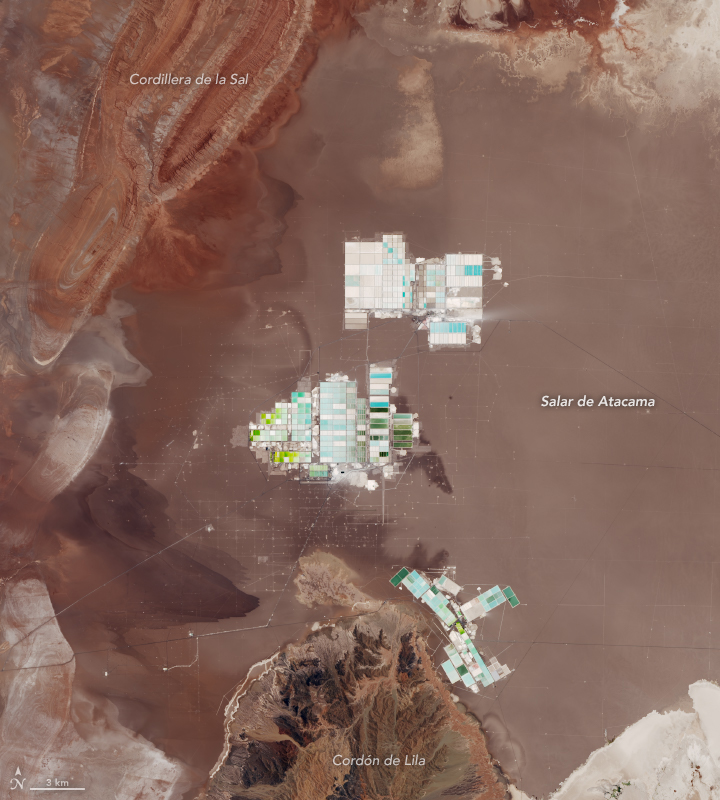
\includegraphics[width=0.48\linewidth]{images/book2/atacama-ponds.jpg}

{\small Bassins d'évaporation de saumure lithinifère sur le salar
d'Atacama, vus de l'espace (Landsat 8, 2018~; NASA Earth Observatory,
domaine public, Wikimedia Commons). La couleur de chaque bassin change à
mesure que la saumure se concentre et que les sels cristallisent.}
\end{omfigure}

\section{L'hydrogène et les hydrures}

L'hydrogène possède un électron~: il peut le perdre (\ce{H+}, porté par
l'eau sous forme de \ce{H3O+}), le mettre en commun (\omterm{def:b1:lewis-resonance-vsepr:lewis}{liaisons
covalentes}) ou en gagner un (\ce{H-}, de \omterm{def:b1:quantum-numbers:configuration}{configuration électronique}
celle de l'hélium). Ce qu'il fait dépend de son partenaire.

\begin{definition}[Hydrures]\label{def:b1:s-block:hydride}
Un \emph{hydrure}\index{hydrure} est un composé binaire de l'hydrogène
et d'un autre élément. Les \emph{hydrures salins}\index{hydrure salin},
formés avec les \omterm{def:b1:s-block:families}{métaux alcalins} et les alcalino-terreux les plus lourds
(\ce{LiH}, \ce{NaH}, \ce{CaH2}), sont des solides ioniques contenant
\ce{H-}. Les \emph{hydrures covalents}\index{hydrure covalent}, formés
avec les éléments du \omterm{def:b1:periodicity:table}{bloc} p (\ce{CH4}, \ce{NH3}, \ce{H2O}, \ce{HCl}),
sont moléculaires. Les \emph{hydrures
métalliques}\index{hydrure metallique@hydrure métallique}, formés avec
certains métaux de transition, sont des solides dans lesquels
l'hydrogène occupe des \omterm{def:b1:crystals-metals:site}{sites interstitiels} du \omterm{def:b1:crystals-metals:lattice}{réseau} du métal, souvent
avec une composition variable.
\end{definition}

L'ion \omterm{def:b1:s-block:hydride}{hydrure} est une base et un \omterm{def:b1:nernst:couple}{réducteur} très forts~: les \omterm{def:b1:s-block:hydride}{hydrures
salins} réagissent avec l'eau, \ce{NaH + H2O -> NaOH + H2}, et servent
d'agents desséchants pour les solvants et de bases en synthèse
organique (\cref{ch:b1:alcohol-activation}).
Les \omterm{def:b1:s-block:hydride}{hydrures covalents} de la deuxième \omterm{def:b1:periodicity:table}{période} traduisent l'évolution de
l'\omterm{def:b1:periodicity:electronegativity}{électronégativité} le long de celle-ci~: \ce{CH4} n'est ni acide ni
basique, \ce{NH3} est basique, \ce{H2O} amphotère, \ce{HF} acide.

\section{Les métaux alcalins}

\begin{definition}[Métaux alcalins et alcalino-terreux]\label{def:b1:s-block:families}
Les \emph{métaux alcalins}\index{metal alcalin@métal alcalin} (Li, Na,
K, Rb, Cs, Fr) forment le \omterm{def:b1:periodicity:table}{groupe} 1, avec un électron de valence
\textit{ns}$^1$~; les \emph{métaux
alcalino-terreux}\index{metal alcalino-terreux@métal alcalino-terreux}
(Be, Mg, Ca, Sr, Ba, Ra) forment le \omterm{def:b1:periodicity:table}{groupe} 2, avec \textit{ns}$^2$. Ces
éléments constituent le \omterm{def:b1:periodicity:table}{bloc} s.
\end{definition}

\begin{proposition}[Les métaux alcalins sont des réducteurs forts]\label{prop:b1:s-block:reducing-power}
Les \omterm{def:b1:s-block:families}{métaux alcalins} ont les \omterm{def:b1:periodicity:ionisation-energy}{énergies de première ionisation} les plus
faibles de leur \omterm{def:b1:periodicity:table}{période} (Li \qty{5.39}{eV}, Na 5.14, K 4.34) et des
\omterm{def:b1:nernst:electrode-potential}{potentiels standard} très négatifs (\ce{Li+}/\ce{Li} $-3.04$~V,
\ce{Na+}/\ce{Na} $-2.71$,
\ce{K+}/\ce{K} $-2.94$)~: ils réduisent l'eau et ne se rencontrent dans
la nature que sous forme d'ions \ce{M+}.
\end{proposition}
% ledger: ie:Li, ie:Na, ie:K (E0 computed in figdata/bachelor-1/standard-potentials.py)

\begin{proof}
Un électron unique à l'extérieur d'un cœur de gaz noble, loin du noyau
et écranté par les couches internes (\cref{ch:b1:periodicity}),
s'arrache facilement. Dans l'eau, le petit ion \ce{M+} est fortement
hydraté, ce qui abaisse encore le potentiel du couple. Avec un
$E^\circ$ inférieur de plus de \qty{2.2}{V} à la droite de l'eau à pH 7
($-0.41$~V), la réaction
\ce{2M + 2H2O -> 2M+ + 2OH- + H2} a une constante énorme
(\cref{prop:b1:nernst:equilibrium-constant}).
\end{proof}

\begin{omfigure}
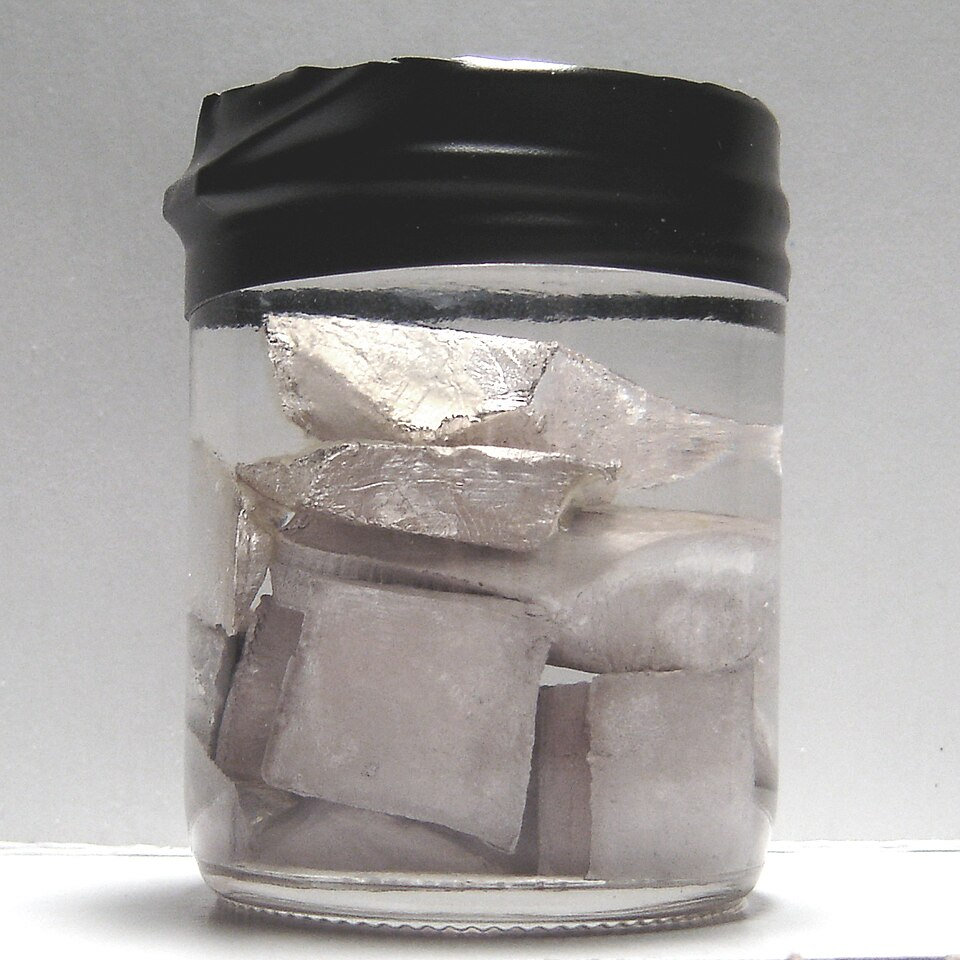
\includegraphics[height=4.6cm]{images/book2/sodium-oil.jpg}\hspace{0.8em}%
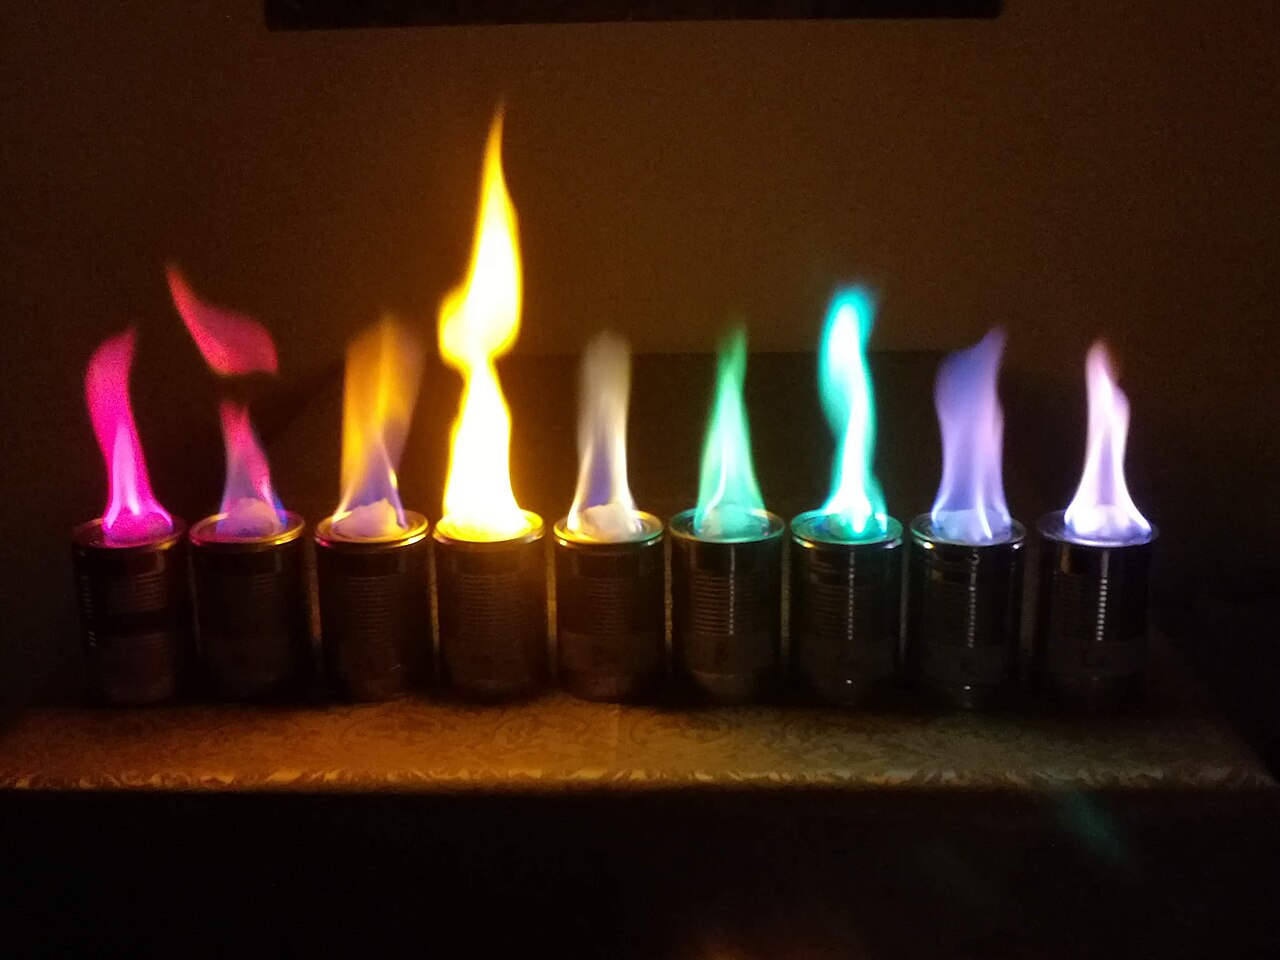
\includegraphics[height=4.6cm]{images/book2/flame-colours.jpg}

{\small À gauche~: le sodium est conservé sous huile minérale, à l'abri
de l'air et de l'humidité (photographie Justin Urgitis, CC BY-SA 2.5). À
droite~: couleurs de flamme, de gauche à droite, de composés du lithium,
du strontium, du calcium, du sodium, du baryum, du bore, du cuivre, du
césium et du potassium~: les électrons excités dans la flamme
retournent vers des niveaux inférieurs en émettant de la lumière à des
longueurs d'onde caractéristiques de chaque élément
(\cref{ch:b1:quantum-numbers}) (photographie Hegelrast, CC BY-SA 4.0).
Les deux images proviennent de Wikimedia Commons.}
\end{omfigure}

\begin{inthelab}[Une démonstration, pas une expérience]
La réaction du sodium avec l'eau n'est montrée que par un enseignant,
derrière un écran de protection, avec un morceau de la taille d'une
lentille lâché dans un grand cristallisoir d'eau additionnée de
phénolphtaléine~: le métal fond en une bille qui court à la surface, le
dihydrogène crépite, et la traînée rose révèle l'hydroxyde formé. Le
potassium enflamme le dihydrogène. De plus gros morceaux explosent. Le
sodium se coupe sous l'huile, se manipule à la pince, et ses résidus
sont détruits à l'éthanol, jamais à l'eau.
\end{inthelab}

Le lithium est l'exception de son groupe~: l'ion le plus petit, le plus
fortement hydraté, donc le potentiel le plus négatif, et pourtant la
réaction la plus lente avec l'eau. Ses composés ressemblent à ceux du
magnésium (le carbonate et le phosphate de lithium sont peu solubles,
comme ceux du magnésium)~: c'est une relation diagonale dans le tableau
périodique. Les \omterm{def:b1:s-block:families}{métaux alcalins} sont produits par électrolyse de leurs
chlorures fondus, car aucun \omterm{def:b1:nernst:couple}{réducteur} chimique n'est assez fort~; les
réactions aux électrodes de ces cellules sont étudiées dans le volume de
deuxième année.

\section{Les composés du sodium dans l'industrie}

\begin{definition}[Caractère des oxydes]\label{def:b1:s-block:oxide-character}
Un \emph{oxyde basique}\index{oxyde basique} réagit avec l'eau pour
donner un hydroxyde, ou avec les acides pour donner des sels (\ce{Na2O},
\ce{CaO})~; un \emph{oxyde acide}\index{oxyde acide} réagit avec l'eau
pour donner un acide, ou avec les bases pour donner des sels (\ce{CO2},
\ce{SO3}, \ce{P4O10})~; un \emph{oxyde amphotère}\index{oxyde amphotere@oxyde amphotère}
réagit à la fois avec les acides et avec les bases (\ce{Al2O3},
\ce{ZnO}). Le long d'une \omterm{def:b1:periodicity:table}{période}, les oxydes passent de basiques
(métaux, à gauche) à acides (non-métaux, à droite).
\end{definition}

L'hydroxyde de sodium est fabriqué par électrolyse de la saumure (le
procédé chlore-soude, qui fournit aussi du dichlore et du dihydrogène).
Le carbonate de sodium, utilisé pour le verre, les détergents et
l'extraction du lithium, est soit extrait sous forme du minéral trona,
soit fabriqué à partir de sel et de calcaire~: en 2025, le monde en a
produit environ 71 millions de tonnes, dont 19 millions issus de
gisements naturels et 52 millions de synthèse, en majeure partie par le
procédé Solvay.
% ledger: usgs:sodaash-total-2025, usgs:sodaash-natural-2025, usgs:sodaash-synthetic-2025

\begin{proposition}[Le procédé Solvay]\label{prop:b1:s-block:solvay}
Le procédé Solvay convertit le chlorure de sodium et le carbonate de
calcium en carbonate de sodium et chlorure de calcium,
\ce{2NaCl + CaCO3 -> Na2CO3 +
CaCl2}, par des étapes dans lesquelles l'ammoniac et le dioxyde de
carbone sont recyclés.
\end{proposition}

\begin{proof}
Les étapes sont~: (1) \ce{CaCO3 -> CaO + CO2} (four à chaux)~;
(2) \ce{NaCl + NH3 +
CO2 + H2O -> NaHCO3 + NH4Cl} (la saumure ammoniacale est carbonatée~;
l'hydrogénocarbonate, le sel le moins soluble présent, précipite)~; (3)
\ce{2NaHCO3 -> Na2CO3 + CO2 + H2O} (calcination)~; (4) \ce{CaO + H2O ->
Ca(OH)2}~; (5) \ce{Ca(OH)2 + 2NH4Cl -> CaCl2 + 2NH3 + 2H2O}
(récupération de l'ammoniac). En additionnant
$(1) + 2\times(2) + (3) + (4) + (5)$, \ce{NH3},
\ce{CO2}, \ce{NH4Cl}, \ce{NaHCO3}, \ce{CaO}, \ce{Ca(OH)2} et l'eau se
simplifient~:
\ce{2NaCl + CaCO3 -> Na2CO3 + CaCl2}.
\end{proof}

\begin{omfigure}
\begin{tikzpicture}[font=\small, >={Stealth}, box/.style={draw, rounded corners, fill=omDef!8, minimum width=2.6cm, minimum height=0.8cm, align=center}]
  \node[box] (kiln) at (0,0) {four à chaux\\\ce{CaCO3 -> CaO + CO2}};
  \node[box] (tower) at (5.3,0) {carbonateur\\\ce{NaHCO3} précipite};
  \node[box] (calc) at (10.2,0) {calcinateur\\\ce{NaHCO3} $\to$ \ce{Na2CO3}};
  \node[box] (slake) at (0,-2.6) {extinction\\\ce{CaO + H2O -> Ca(OH)2}};
  \node[box] (still) at (5.3,-2.6) {distillateur\\\ce{NH4Cl + Ca(OH)2}};
  \draw[->, thick] (kiln) -- node[above] {\ce{CO2}} (tower);
  \draw[->, thick] (tower) -- node[above, font=\scriptsize] {\ce{NaHCO3}} (calc);
  \draw[->, thick] (calc.north) -- ++(0,0.6) -| node[pos=0.25, above] {\ce{CO2} recyclé} (tower.north);
  \draw[->, thick] (kiln) -- node[left] {\ce{CaO}} (slake);
  \draw[->, thick] (slake) -- node[above, font=\scriptsize] {\ce{Ca(OH)2}} (still);
  \draw[->, thick] (tower) -- node[right] {\ce{NH4Cl}} (still);
  \draw[->, thick] (still.east) -- ++(1.2,0) |- node[pos=0.25, right] {\ce{NH3} recyclé} ($(tower.east)+(0,-0.25)$);
  \draw[<-, thick] (tower.north west) -- ++(-0.5,0.6) node[above] {saumure \ce{NaCl}};
  \draw[->, thick] (calc.east) -- ++(0.8,0) node[right] {\ce{Na2CO3}};
  \draw[->, thick] (still.south) -- ++(0,-0.6) node[below] {\ce{CaCl2}};
\end{tikzpicture}

{\small Le procédé Solvay. Le dioxyde de carbone et l'ammoniac
circulent en boucle~; le sel et le calcaire entrent, le carbonate de
sodium et le chlorure de calcium sortent.}
\end{omfigure}

\begin{omfigure}
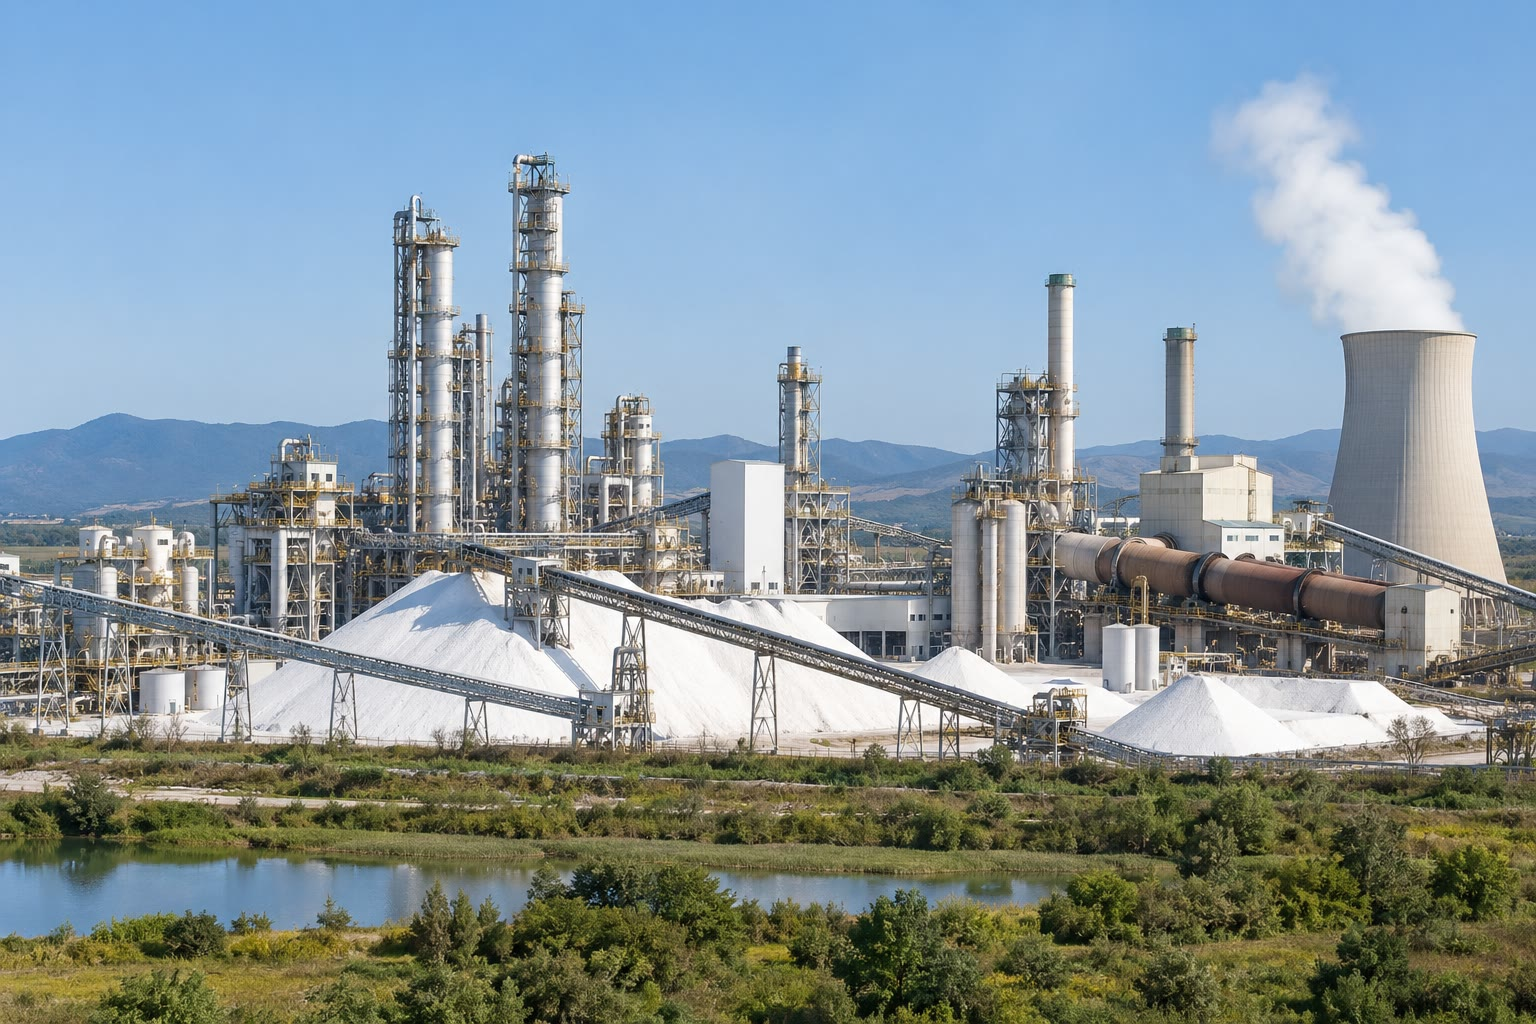
\includegraphics[width=0.55\linewidth]{images/book2/ai/b1-26-soda-ash-plant.jpg}

{\small Une usine de carbonate de sodium~: fours à chaux, tours de
carbonatation et stocks de carbonate de sodium.}
\end{omfigure}

\begin{method}[Bilan de matière sur un schéma de procédé]\label{met:b1:s-block:mass-balance}
\begin{enumerate}
  \item Écrire l'équation globale (somme des étapes, espèces recyclées
        simplifiées).
  \item À partir du produit voulu, calculer les quantités de matières
        premières avec l'équation globale, puis corriger du \omterm{def:b1:extent-q-and-k:fractional-extent}{rendement} de
        chaque étape.
  \item Pour une espèce recyclée, ne calculer que l'appoint nécessaire
        pour compenser ses pertes.
  \item Vérifier le bilan de chaque élément entre entrées et sorties.
\end{enumerate}
\end{method}

\section{Les métaux alcalino-terreux}

Le magnésium et le calcium sont moins réactifs que les \omterm{def:b1:s-block:families}{métaux alcalins}
(énergies d'ionisation plus élevées~: Mg \qty{7.65}{eV}, Ca 6.11~; deux
électrons à perdre), mais restent des \omterm{def:b1:nernst:couple}{réducteurs} forts ($E^\circ$ de
\ce{Mg^2+}/\ce{Mg} $-2.36$~V).
Le magnésium brûle dans l'air avec une lumière blanche éblouissante~; sa
couche d'oxyde le protège à température ambiante. On récupère le
magnésium de l'eau de mer en précipitant son hydroxyde par la chaux,
$\mathrm{p}K_s = 11.25$
(\cref{ch:b1:precipitation}).
% ledger: ie:Mg, ie:Ca

\begin{proposition}[Le cycle de la chaux]\label{prop:b1:s-block:lime-cycle}
Calcaire, chaux vive, chaux éteinte et de nouveau calcaire forment un
cycle~:
\ce{CaCO3 -> CaO + CO2} (chauffage dans un four)~; \ce{CaO + H2O -> Ca(OH)2}
(extinction, fortement exothermique)~; \ce{Ca(OH)2 + CO2 -> CaCO3 + H2O}
(prise du mortier de chaux à l'air). Le cycle dans son ensemble ne change
rien chimiquement, mais stocke et libère de l'énergie et du dioxyde de
carbone.
\end{proposition}

\begin{proof}
En additionnant les trois équations, toutes les espèces se simplifient.
La décomposition du carbonate exige de la chaleur, restituée lors des
deux autres étapes~; le \ce{CO2} dégagé dans le four est repris,
lentement, par le mortier.
\end{proof}

\begin{omfigure}
\begin{tikzpicture}[font=\small, >={Stealth}]
  \node[draw, rounded corners, fill=omDef!8] (a) at (90:2.0) {\ce{CaCO3} calcaire};
  \node[draw, rounded corners, fill=omDef!8] (b) at (-30:2.0) {\ce{CaO} chaux vive};
  \node[draw, rounded corners, fill=omDef!8] (c) at (210:2.0) {\ce{Ca(OH)2} chaux éteinte};
  \draw[->, thick] (a) to[bend left=25] node[right, align=left] {chauffage\\$-\ce{CO2}$} (b);
  \draw[->, thick] (b) to[bend left=25] node[below] {$+\ce{H2O}$} (c);
  \draw[->, thick] (c) to[bend left=25] node[left, align=right] {$+\ce{CO2}$\\$-\ce{H2O}$} (a);
\end{tikzpicture}

{\small Le cycle de la chaux, du calcaire au mortier et retour au
carbonate de calcium.}
\end{omfigure}

\section{Le lithium}

\begin{omfigure}
\begin{tikzpicture}
\begin{axis}[
  xbar, width=0.78\linewidth, height=5.4cm, xmin=0, xmax=110,
  symbolic y coords={CA,ML,BR,AR,ZW,CL,CN,AU}, ytick=data,
  yticklabels={Canada, Mali, Brésil, Argentine, Zimbabwe, Chili, Chine, Australie},
  xlabel={lithium extrait en 2025 (milliers de tonnes de Li, estimations)}, bar width=8pt,
  nodes near coords, every node near coord/.append style={font=\scriptsize},
  tick label style={font=\small}, label style={font=\small}, enlarge y limits=0.1]
\addplot[fill=omDef!45, draw=omDef] coordinates {(5.6,CA) (9.4,ML) (12,BR) (23,AR) (28,ZW) (56,CL) (62,CN) (92,AU)};
\end{axis}
\end{tikzpicture}

{\small Les principaux producteurs de lithium en 2025 (estimations~;
total mondial d'environ \num{290000} tonnes de lithium). L'Australie
exploite des roches dures (spodumène)~; le Chili et l'Argentine pompent
des saumures.}
% ledger: usgs:li-canada-2025, usgs:li-mali-2025, usgs:li-brazil-2025, usgs:li-argentina-2025, usgs:li-zimbabwe-2025, usgs:li-chile-2025, usgs:li-china-2025, usgs:li-australia-2025, usgs:li-world-2025
\end{omfigure}

La saumure est concentrée par évaporation, le magnésium éliminé par la
chaux, et le carbonate de lithium précipité par le carbonate de sodium.
Le carbonate de lithium a la propriété inhabituelle d'être moins soluble
à chaud qu'à froid~: \qty{1.31}{\percent}
en masse à \qty{20}{\celsius}, \qty{0.84}{\percent} à \qty{80}{\celsius},
\qty{0.71}{\percent} à \qty{100}{\celsius}. On le précipite donc à
chaud, comme le calcule le problème du week-end.
% ledger: sol:Li2CO3-20, sol:Li2CO3-80, sol:Li2CO3-100

\section{Exercices}

\begin{exercise}[$\star$]\label{exo:b1:s-block:1}
Classer en \omterm{def:b1:s-block:hydride}{hydrure salin}, covalent ou métallique~: \ce{KH}, \ce{SiH4},
\ce{CaH2}, \ce{H2S}, \ce{PdH_{0.6}}. Écrire la réaction de \ce{CaH2} avec l'eau.
\end{exercise}

\begin{exercise}[$\star$]\label{exo:b1:s-block:2}
Écrire les réactions du lithium, du sodium et du potassium avec l'eau,
et du magnésium avec l'acide chlorhydrique dilué.
\end{exercise}

\begin{exercise}[$\star$]\label{exo:b1:s-block:3}
Classer en \omterm{def:b1:s-block:oxide-character}{oxyde basique}, acide ou amphotère~: \ce{Na2O}, \ce{MgO}, \ce{Al2O3},
\ce{SiO2}, \ce{SO3}, \ce{ZnO}, \ce{CO2}. Écrire une réaction pour chaque
catégorie.
\end{exercise}

\begin{exercise}[$\star$]\label{exo:b1:s-block:4}
Calculer la constante de \ce{2Na + 2H2O -> 2Na+ + 2OH- + H2} à pH 14 à
partir des \omterm{def:b1:nernst:electrode-potential}{potentiels standard}.
\end{exercise}

\begin{exercise}[$\star\star$]\label{exo:b1:s-block:5}
Expliquer les couleurs de flamme du lithium (rouge) et du sodium (jaune)
à l'aide des \omterm{def:b1:quantum-numbers:energy-level}{niveaux d'énergie} des atomes (\cref{ch:b1:quantum-numbers}).
Quelle est l'énergie d'un photon jaune à \qty{589}{nm}~?
\end{exercise}

\begin{exercise}[$\star\star$]\label{exo:b1:s-block:6}
Calculer la masse de calcaire (\ce{CaCO3} pur) et de chlorure de sodium
nécessaire pour une tonne de carbonate de sodium par le procédé Solvay,
avec un \omterm{def:b1:extent-q-and-k:fractional-extent}{rendement} global de \qty{90}{\percent} sur le chlorure de
sodium.
\end{exercise}

\begin{exercise}[$\star\star$]\label{exo:b1:s-block:7}
L'eau de mer contient environ \qty{1.3}{g/L} de magnésium (donnée de
l'exercice). À quel pH l'hydroxyde de magnésium commence-t-il à
précipiter~? Quelle masse de chaux éteinte précipite le magnésium de
\qty{1.0}{m^3}~?
\end{exercise}

\begin{exercise}[$\star\star$]\label{exo:b1:s-block:8}
Pourquoi le lithium réagit-il plus lentement avec l'eau que le
potassium, bien que son \omterm{def:b1:nernst:electrode-potential}{potentiel standard} soit plus bas~? Distinguer
thermodynamique et cinétique.
\end{exercise}

\begin{exercise}[$\star\star$]\label{exo:b1:s-block:9}
Calculer la masse de chaux vive obtenue à partir d'une tonne de calcaire
et le volume de \ce{CO2} dégagé, à \qty{25}{\celsius} et \qty{1}{bar}.
\end{exercise}

\begin{exercise}[$\star\star\star$]\label{exo:b1:s-block:10}
Le monde a extrait environ \num{290000} tonnes de lithium en 2025. À
quelle masse de carbonate de lithium cela correspond-il~? Si une
batterie de voiture contient \qty{8}{kg} de
lithium (donnée de l'exercice), combien de batteries cela
permettrait-il d'équiper~?
\end{exercise}

\begin{exercise}[$\star\star\star$]\label{exo:b1:s-block:11}
Montrer à partir des données du chapitre que la \omterm{def:b1:precipitation:solubility}{solubilité} du carbonate
de lithium diminue quand la température augmente, et expliquer pourquoi
le précipiter à chaud améliore le \omterm{def:b1:extent-q-and-k:fractional-extent}{rendement} d'extraction à partir d'une
saumure.
\end{exercise}

\begin{exercise}[$\star\star\star$]\label{exo:b1:s-block:12}
À l'étape (2) du procédé Solvay, la solution contient \ce{Na+},
\ce{NH4+}, \ce{Cl-} et \ce{HCO3-}. Expliquer pourquoi c'est
l'hydrogénocarbonate de sodium qui précipite et non le chlorure
d'ammonium, et pourquoi le procédé exige l'ammoniac plutôt que
l'hydroxyde de sodium.
\end{exercise}

% fr layout: the problem box fills a page and cannot break under its
% heading, so the page is opened and slightly enlarged to hold both
\clearpage
\enlargethispage{3\baselineskip}
\section{Problème~: le lithium des saumures}

\begin{problem}[{Problème du week-end --- concentrer une saumure de
lithium, éliminer le magnésium par la chaux, précipiter le carbonate de
lithium par le carbonate de sodium, et la masse de carbonate de lithium
récupérée à partir d'un mètre cube}]
\label{pb:b1:s-block:1}
Une saumure pompée sous un salar contient \qty{1.5}{g/L} de lithium
et \qty{0.60}{g/L} de magnésium (sous forme d'ions, avec beaucoup de
chlorure de sodium). L'évaporation en bassins la concentre quatre fois.
Un mètre cube de la saumure concentrée est ensuite traité~: la chaux
élimine le magnésium, le carbonate de sodium le calcium, et du carbonate
de sodium chaud précipite enfin le carbonate de lithium à
\qty{80}{\celsius}. Données~: masses molaires (\unit{g/mol}) Li 6.9, Mg 24.3,
\ce{Ca(OH)2} 74.1, \ce{Na2CO3} 106.0, \ce{Li2CO3} 73.8~; $\mathrm{p}K_s$
\ce{Mg(OH)2} 11.25, \ce{CaCO3} 8.30~; $\mathrm{p}K_e = 14.00$~;
\omterm{def:b1:precipitation:solubility}{solubilité} de \ce{Li2CO3} \qty{0.84}{\percent} en masse à
\qty{80}{\celsius}~; on assimile la liqueur finale à \qty{1.00}{m^3} de
masse volumique \qty{1.0}{kg/L}.

\medskip
\noindent\textbf{Partie I --- La concentration.}
\begin{enumerate}
  \item Calculer les concentrations du lithium et du magnésium dans la
        saumure concentrée.
  \item Quel volume d'eau s'évapore par mètre cube de saumure
        concentrée~?
  \item Pourquoi utilise-t-on l'évaporation solaire plutôt qu'un
        chauffage~?
  \item Quel sel cristallise en premier dans les bassins, et pourquoi~?
  \item Calculer les quantités de matière de lithium et de magnésium dans
        un mètre cube.
  \item Pourquoi faut-il éliminer le magnésium avant de précipiter le
        lithium~?
\end{enumerate}

\medskip
\noindent\textbf{Partie II --- Éliminer le magnésium et le calcium.}
\begin{enumerate}[resume]
  \item Écrire la réaction des ions magnésium avec la chaux éteinte.
  \item Calculer la masse de chaux éteinte nécessaire
        (stœchiométrique).
  \item À quel pH \qty{99.9}{\percent} du magnésium sont-ils
        précipités~?
  \item Pourquoi le lithium ne précipite-t-il pas sous forme
        d'hydroxyde~?
  \item Écrire l'élimination du calcium introduit, par le carbonate de
        sodium.
  \item Calculer la masse de carbonate de sodium nécessaire à cette
        étape.
\end{enumerate}

\medskip
\noindent\textbf{Partie III --- Le carbonate de lithium.}
\begin{enumerate}[resume]
  \item Écrire la précipitation du carbonate de lithium.
  \item Calculer la masse de carbonate de sodium nécessaire pour le
        lithium.
  \item Calculer la masse théorique de carbonate de lithium.
  \item Pourquoi la précipitation est-elle réalisée à
        \qty{80}{\celsius}~?
  \item Quelle masse de carbonate de lithium reste dissoute dans la
        liqueur~?
  \item Comment lave-t-on le précipité sans en perdre beaucoup~?
\end{enumerate}

\medskip
\noindent\textbf{Partie IV --- Le bilan.}
\begin{enumerate}[resume]
  \item Calculer la masse de carbonate de lithium récupérée.
  \item Calculer le taux de récupération du lithium.
  \item Proposer un usage de la liqueur.
  \item Comparer le lithium d'un mètre cube à la production mondiale de
        2025~: combien de mètres cubes cette production
        représenterait-elle~?
  \item Donner la masse de carbonate de lithium récupérée par mètre cube
        de saumure concentrée.
\end{enumerate}
\end{problem}
